\section{Temporal Graph Reasoning Benchmark: \benchmarkname \raisebox{-1mm}{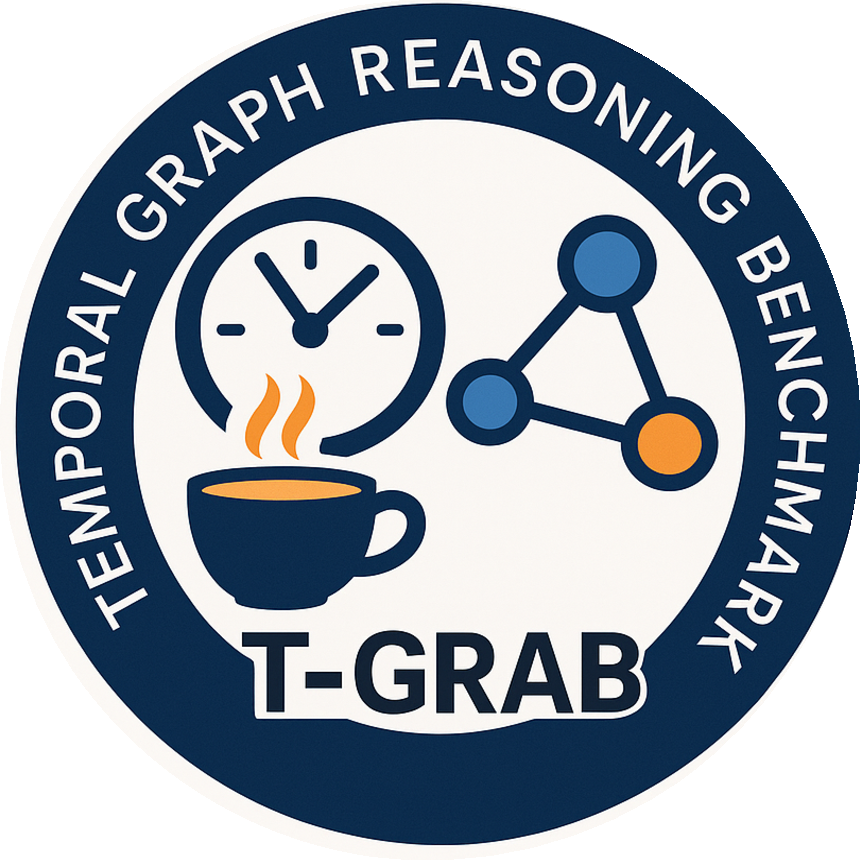
\includegraphics[height=1.5em]{figs/logo.pdf}
 }}\label{sec:tgrab}


\looseness-1 In this section, we introduce the Temporal Graph Reasoning Benchmark~(\benchmarkname), the first synthetic dataset to systematically diagnose the capabilities of TGNNs to reason over time in a controlled environment. In \benchmarkname, we include three sets of dynamic link prediction tasks: 1) the \emph{periodicity} tasks which probes the counting/memorization capabilities of TGNNs, 2) the \emph{cause-and-effect} tasks which gauges how well TGNNs can infer delayed cause-and-effect patterns, and 3) the \emph{long-range spatio-temporal} tasks to measure the ability of TGNNs to capture long-range dependencies across spatial and temporal dimensions. The \emph{periodicity} tasks, the \emph{cause-and-effect} task and the \emph{long-range spatio-temporal} tasks are discussed in detail in Section~\ref{synth-benchmark:periodicity}, ~\ref{synth-benchmark:cause}, ~\ref{synth-benchmark:long} respectively. \Cref{tab:data} provides an overview of the statistics of the tasks introduced in \benchmarkname, revealing a diverse range of task characteristics to test the limits of TGNNs.

\begin{table*}[t]
\caption{\benchmarkname dataset statistics and characteristics. } \label{tab:data} 
  \resizebox{\linewidth}{!}{%
  \begin{tabular}{ l | cccccc}
  \toprule
  Dataset & \# Nodes & \# Edges
  & \# Timestamp & Counting & Memorizing & \begin{tabular}{cc}
       Spatial  \\ Understanding
  \end{tabular}  \\ 
  \midrule
  Periodicity &  100 & 10,560 - 9,144,440 & 96 - 12,288 & \cmark & \cmark & \xmark\\ 
  Cause-and-Effect &  101 & 164,856 - 174,470 & 4,001 - 4,256 & \xmark & \cmark & \xmark\\ 
  Long-Range Spatio-Temporal &  102 & 48,006 - 411,072 & 4,001 - 4,032 & \xmark & \cmark & \cmark\\ 
  \bottomrule
  \end{tabular}
  }
\end{table*}

% Table~\ref{tab:data} provides an overview of the statistics and characteristics of the datasets introduced in \benchmarkname. Table~\ref{tab:data} shows that \benchmarkname covers a diverse range of dataset statistics and associated tasks to test the limit of TGNNs.

\looseness-1 \textbf{Methods in Comparison.} We compare a range of Temporal Graph Learning (TGL) methods  on \benchmarkname's tasks
%~(experimental details can be found in \Cref{appendix:experimental-details})
: four continuous-time~(CTDG) methods~(DyGFormer~\cite{dygformer}, CTAN~\cite{ctan}, TGN~\cite{tgn} and TGAT~\cite{tgat}), three discrete-time~(DTDG) methods~(EvolveGCN~\cite{evolvegcn}, T-GCN~\cite{tgcn}, and GC-LSTM~\cite{gclstm}), two static graph methods~(GCN~\citep{gcn} and GAT~\cite{gat}), and two baselines~(\textit{persistence}, which always predicts the edges present at the previous time step, and $\text{Edgebank}_{\infty}$\citep{poursafaei2022betterevaluationdynamiclink}). 
%Model sizes are detailed in Appendix~\ref{appendix:parameters}.

% \ah{we need to add some details of how we apply CTDG methods on DTDG datasets. We can discuss here if we have space or put it in experiment details.}
% \gr{There is one or two small sentences at the end of Sec 3 about this, we can add more details in appendix indeed.  }


\textbf{Evaluation Protocols.}
It was shown that different negative samples can cause significant differences in evaluation results for dynamic link prediction~\cite{poursafaei2022betterevaluationdynamiclink}. To mitigate this, we opt for the most robust evaluation where we evaluate models using the average $F_1$ score over all possible node pairs at each test time step. For periodicity tasks, all test edges are included in the $F_1$ calculation. In contrast, for the cause-and-effect and long-range tasks, only edges involving the memory/target node are considered, as all other edges are randomly generated and thus unpredictable. 

% Since the dynamic graphs we consider are relatively small, we do not have to rely on negative sampling for our evaluation, which has many drawbacks~\cite{poursafaei2022betterevaluationdynamiclink}, and instead evaluate the models by reporting the average $F_1$ score over all possible edges across all time steps in the test set.  For the periodicity tasks, all edges in the test set are included in the $F_1$ computation. For the  cause and effect and long range tasks, not all edges are included in the $F_1$ computation since only the edges involving the memory node can be predicted. Indeed, all the other edges are generated completely at random. Hence, for these tasks the $F_1$ is averaged only over the edges of the test set involving the memory node. 